% ------------------------------------------------------------------------------
% TYPO3 CMS 7.3 - What's New - Chapter "Introduction" (English Version)
%
% @author	Michael Schams <schams.net>
% @license	Creative Commons BY-NC-SA 3.0
% @link		http://typo3.org/download/release-notes/whats-new/
% @language	English
% ------------------------------------------------------------------------------
% LTXE-CHAPTER-UID:		066dde91-8cd613b5-0eadb76c-a6245b74
% LTXE-CHAPTER-NAME:	Introduction
% ------------------------------------------------------------------------------

\section{Introduzione}
\begin{frame}[fragile]
	\frametitle{Introduzione}

	\begin{center}\huge{Introduzione}\end{center}
	\begin{center}\huge{\color{typo3darkgrey}\textbf{I fatti in breve}}\end{center}

\end{frame}

% ------------------------------------------------------------------------------
% LTXE-SLIDE-START
% LTXE-SLIDE-UID:		7a129462-c5d593ea-6faef810-b616bc9e
% LTXE-SLIDE-ORIGIN:	1c3389b6-2103f93f-b2319a3e-aacc6eba English
% LTXE-SLIDE-ORIGIN:	6d5e9f3e-f9d9677e-43d7d497-e80ba9ef German
% LTXE-SLIDE-TITLE:		TYPO3 CMS 7.3 - The Facts
% ------------------------------------------------------------------------------
\begin{frame}[fragile]
	\frametitle{Introduzione}
	\framesubtitle{TYPO3 CMS 7.3 - I fatti in breve}

	\begin{itemize}
		\item Data di rilascio: 16 giugno 2015
		\item Tipo di rilascio: "Sprint Release"
		\item Visione: Embrace, Innovate, Deliver
		\item Focus principale: Ecosistema Pacchetti, Composer e gestione estensioni
	\end{itemize}

\end{frame}

% ------------------------------------------------------------------------------
% LTXE-SLIDE-START
% LTXE-SLIDE-UID:		2fbf0553-2a21cfa2-58045b63-43df3438
% LTXE-SLIDE-ORIGIN:	780b1e6f-e761ec98-824890a3-8d429b56 English
% LTXE-SLIDE-ORIGIN:	759c3860-d5061f6e-2bb0009f-6ea130c8 German
% LTXE-SLIDE-TITLE:		System Requirements
% ------------------------------------------------------------------------------
\begin{frame}[fragile]
	\frametitle{Introduzione}
	\framesubtitle{Requisiti di sistema}

	\begin{itemize}
		\item PHP*:\tabto{2.2cm}v5.5.0 - v5.6.x
		\item MySQL:\tabto{2.2cm}v5.5.x - v5.6.x (no strict mode)
		\item Spazio disco:\tabto{2.2cm}min 200 MB
		\item Impostazioni PHP:

			\begin{itemize}
				\item memory\_limit >= 128M
				\item max\_execution\_time >= 240s
				\item l'opzione di compilazione \texttt{--disable-ipv6} \underline{non} deve essere usata
			\end{itemize}

		\item Il Backend richiede IE >= 9 o qualsiasi altro browser moderno

	\end{itemize}

	\vspace{1cm}
	*) Altri dettagli: \href{http://typo3.org/news/article/php-minimum-requirements-for-typo3-cms-7/}{Requisiti minimi PHP per TYPO3 CMS 7}

\end{frame}

% ------------------------------------------------------------------------------
% LTXE-SLIDE-START
% LTXE-SLIDE-UID:		12de4c00-b5f6cb41-1043baf0-b07911da
% LTXE-SLIDE-ORIGIN:	e06c97c6-ee283664-40fe3fe5-af3a1caa English
% LTXE-SLIDE-ORIGIN:	70c77c41-e2b83d82-2f182996-98061070 German
% LTXE-SLIDE-TITLE:		Development And Release Timeline
% ------------------------------------------------------------------------------
\begin{frame}[fragile]
	\frametitle{Introduzione}
	\framesubtitle{Sviluppo e tempi di rilascio}

	\begin{figure}
		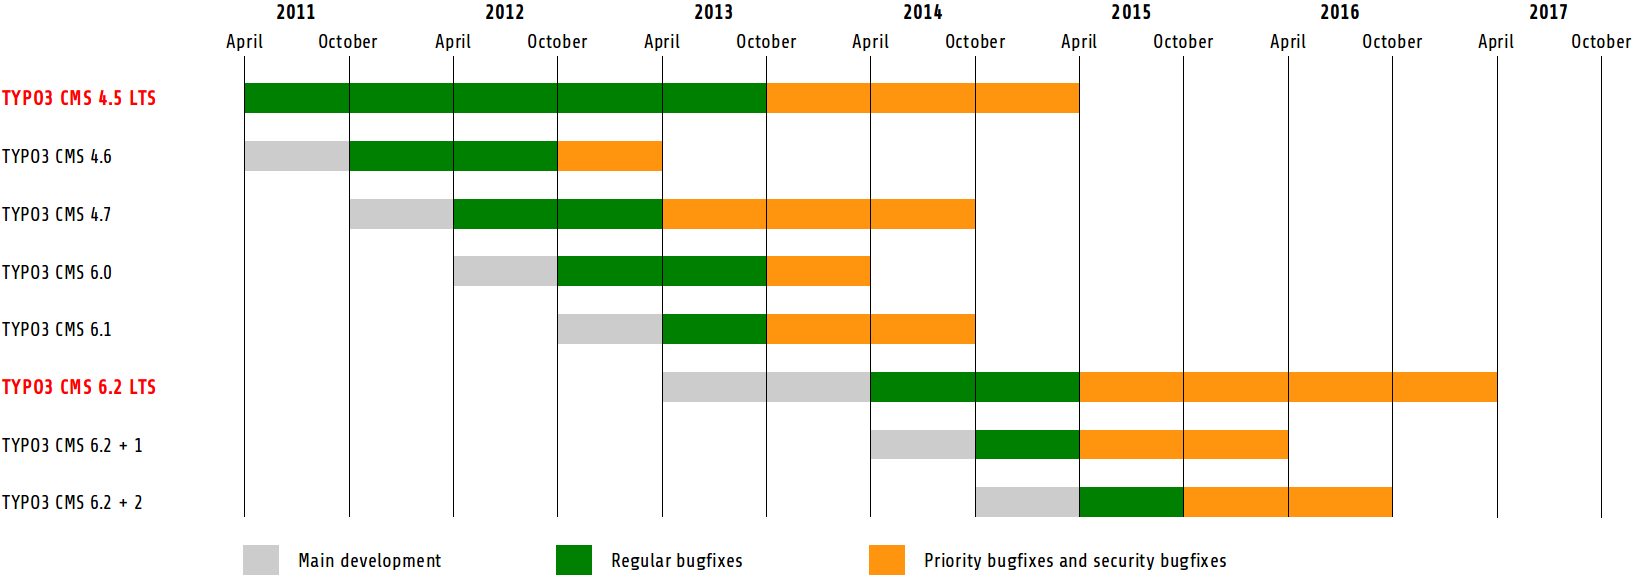
\includegraphics[width=0.90\linewidth]{Introduction/ReleaseAgenda.png}
	\end{figure}

\end{frame}

% ------------------------------------------------------------------------------
% LTXE-SLIDE-START
% LTXE-SLIDE-UID:		5cb3a7fb-be288241-2b7ed7da-932e5e2e
% LTXE-SLIDE-ORIGIN:	cfdf68b1-b00a3fca-0adf0630-7563d7da English
% LTXE-SLIDE-ORIGIN:	b55d3fe9-76807061-d97f3fee-7db1f190 German
% LTXE-SLIDE-TITLE:		TYPO3 CMS Roadmap
% ------------------------------------------------------------------------------
\begin{frame}[fragile]
	\frametitle{Introduzione}
	\framesubtitle{TYPO3 CMS Roadmap}

	Date di rilascio stimate e loro obiettivo principale:

	\begin{itemize}
		\item v7.0 \tabto{1.0cm}02/Dec/2014\tabto{3.4cm}Revisione Backend Vol. 1
		\item v7.1 \tabto{1.0cm}24/Feb/2015\tabto{3.4cm}Pulizia core \& ottimizzazioni
		\item v7.2 \tabto{1.0cm}28/Apr/2015\tabto{3.4cm}Frontend

		\item
			\begingroup
				\color{typo3orange}
					v7.3 \tabto{1.0cm}16/Jun/2015\tabto{3.4cm}Ecosistema Pacchetti, Composer\newline
					\tabto{3.4cm}e gestione estensioni
			\endgroup

		\item v7.4 \tabto{1.0cm}04/Aug/2015\tabto{3.4cm}Revisione Backend Vol. 2
		\item v7.5 \tabto{1.0cm}29/Sep/2015\tabto{3.4cm}\textit{(da determinare...)}
		\item v7.6 \tabto{1.0cm}xx/xxx/2015\tabto{3.4cm}\textbf{TYPO3 CMS 7 LTS} (Long Term Release)
	\end{itemize}

	\smaller
		\url{https://typo3.org/typo3-cms/roadmap/}\newline
		\url{http://typo3.org/news/article/embrace-and-innovate-typo3-cms-7/}
	\normalsize

\end{frame}

% ------------------------------------------------------------------------------
% LTXE-SLIDE-START
% LTXE-SLIDE-UID:		96f5f675-bbfcbb4e-03207178-eba64fda
% LTXE-SLIDE-ORIGIN:	eb02037c-0fba04b6-5006d3f3-03fe223a English
% LTXE-SLIDE-ORIGIN:	b0c28f26-c3ca2e99-195954a8-ed76f9d4 German
% LTXE-SLIDE-TITLE:		Installation
% ------------------------------------------------------------------------------
\begin{frame}[fragile]
	\frametitle{Introduzione}
	\framesubtitle{Installazione}

	\begin{itemize}
		\item Procedura ufficiale di installazione su Linux/Mac OS X\newline
			(DocumentRoot ad esempio \texttt{/var/www/site/htdocs}):
		\begin{lstlisting}
			$ cd /var/www/site
			$ wget --content-disposition get.typo3.org/7.3
			$ tar xzf typo3_src-7.3.0.tar.gz
			$ cd htdocs
			$ ln -s ../typo3_src-7.3.0 typo3_src
			$ ln -s typo3_src/index.php
			$ ln -s typo3_src/typo3
			$ touch FIRST_INSTALL
		\end{lstlisting}

		\item Link simbolici in Microsoft Windows:

			\begin{itemize}
				\item Use \texttt{junction} in Windows XP/2000
				\item Use \texttt{mlink} in Windows Vista and Windows 7
			\end{itemize}

	\end{itemize}
\end{frame}

% ------------------------------------------------------------------------------
% LTXE-SLIDE-START
% LTXE-SLIDE-UID:		3c42f268-691797f7-bfe83767-021876c2
% LTXE-SLIDE-ORIGIN:	5c2e0134-2f1f18d2-55b74162-25dd3995 English
% LTXE-SLIDE-ORIGIN:	48136734-ae508d23-bce5811d-667f8908 German
% LTXE-SLIDE-TITLE:		Upgrade to TYPO3 CMS 7
% ------------------------------------------------------------------------------
\begin{frame}[fragile]
	\frametitle{Introduzione}
	\framesubtitle{Aggiornamento a TYPO3 CMS 7.x}

	\begin{itemize}
		\item Aggiornamenti possibili solo da TYPO3 CMS 6.2 LTS
		\item TYPO3 CMS < 6.2 deve essere prima aggiornato a TYPO3 CMS 6.2 LTS
	\end{itemize}

	\begin{itemize}

		\item Istruzioni per l'aggiornamento:\newline
			\smaller\url{http://wiki.typo3.org/Upgrade#Upgrading_to_7.3}\normalsize
		\item Guida ufficiale TYPO3 "TYPO3 Installation and Upgrading":
			\smaller\url{http://docs.typo3.org/typo3cms/InstallationGuide}\normalsize
		\item Approcio generale:
			\begin{itemize}
				\item Verifica i requisiti minimi di sistema \small(PHP, MySQL, etc.)
				\item Verifica \textbf{deprecation\_*.log} nella vecchia istanza TYPO3
				\item Aggiorna tutte le estensioni all'ultima versione
				\item Imposta il nuovo sorgente ed esegui Install Tool \textrightarrow Upgrade Wizard
				\item Verifica modulo startup per gli utente di backend (opzionale)
			\end{itemize}
	\end{itemize}

\end{frame}

% ------------------------------------------------------------------------------
